\chapter{Lernskript}
\section{Java-Editionen}
	\begin{itemize}
	\item Java läuft auf sehr unterschiedlichen Systemen
	\item  Wird in verschiedenen „Packungsgrößen“ angeboten
	\begin{itemize}
		\item EE (enterprise edition): große Unternehmensserver
		\item SE (standard edition): Desktop-Systeme
		\item ME (micro edition): Handys, PDAs, Embedded Systems
	\end{itemize}
	\item Editionen unterscheiden sich in den mitgelieferten Zugaben,nicht in der Programmiersprache
	\end{itemize}
%
%
%
\section{Java-Entwicklungssystem}
\begin{itemize}
\item Zum Schreiben neuer Programm ist der Compiler javac nötig, zum Ausführen fertiger Programm nicht
\item  Java für verschiedene Einsatzzwecke:
	\begin {itemize}
		\item JRE (java runtime environment): zum Ausführen fertiger Programme
		\item JDK (java development kit): JRE + Compiler und weitere Hilfsmittel zum Schreiben neuer Programme
	\end{itemize}
\end{itemize}
 %
 %
 %
 \section{Namen in Java}
 \begin{itemize}
 \item An vielen Stellen frei wählbare Namen = „Bezeichner“, „Identifier“
 \item Bestandteile: Große und kleine Buchstaben, Ziffern, Underscore (\_)
 \item Erstes Zeichen darf keine Ziffer sein
 \item Etwa fünfzig reservierte Wörter dürfen nicht als Identifier benutzt werden (beispielsweise class, int, public)
	 \item Beispiele:
 	\begin{itemize}
		\item Counter
		\item colorDepth
		\item Iso9660
		\item XMLProcessor
		\item MAX\_VALUE
	\end{itemize}
	\item Nicht erlaubt sind z.B.:
	\begin{itemize}
		\item1stTry 	(erster Buchstabe darf keine Ziffer sein)
		\item Herz Dame (Leerzeichen im Namen nicht erlaubt)
		\item const (reserviertes Wort)
		\item muenchen-erding (Bindestrich im Namen nicht erlaubt)
	\end{itemize}
	\item Übliche Konventionen für Java-Identifier:
	\begin{itemize}
		\item Variablen, Methoden, primitive Typen: CamelCode, erster Buchstabe klein: counter, find1stToken, bottomUp
 		\item Referenztypen: CamelCode, erster Buchstabe groß: Hello, String, ServerSocket
		\item Typvariablen (Generics): einzelne große Buchstaben: T, U
		\item statische, öffentliche Konstanten: alle Buchstaben groß, Wortteile getrennt mit Underscore: MAX\_VALUE, PI, RGB24
	\end{itemize}
\end{itemize}
%
%
%
\section{Regel Ebenen}
\subsection{Syntax (Rechtschreibung)}
Verteilung von Semikolons, Klammern, Schreibweise von Namen
\subsubsection{Syntaxfehler}
Compiler meldet einen Fehler

\subsection{Semantik (Bedeutung)}
Zulässige Kombination von Sprachelementen
\subsubsection{Semantikfehler}
Compiler meldet einen Fehler, Programm verhält sich falsch, stürzt
nach dem Start ab, ...

\subsection{Pragmatik (Gebrauch)}
Bewährte und sinnvolle Konstruktionen
\subsubsection{Fehler der Pragmatik}
Programm ist unleserlich, umständlich, unverständlich
%
%
%
\section{Polymorphismus}
\begin{itemize}
	\item Der Typ des Ergebnisses, und u.U. der Wert, ist abhängig von
	den Typen der Operanden:
	\begin{description}
		\item []$ 20/8 \rightarrow 2 $
		\item []$20.0/8.0 \rightarrow 2.5$
	\end{description}
	\item Zwei Operanden gleichen Typs: Operandentyp = Ergebnistyp
	\item Gemischte Operandentypen: double-Ergebnis:
	\begin{description}
		\item [] $1 + 2 \rightarrow 3$ (int)
		\item [] $1.0 + 2 \rightarrow 3.0$ (double)
		\item[] $1 + 2.0 \rightarrow 3.0$ (double)
		\item[] $1.0+2.0 \rightarrow 3.0$ (double)
	\end{description}
\end{itemize}
%
%
%
\section{Explizite Typkonversionen}
\begin{itemize}
	\item Hohe Priorität, wie andere unäre Operatoren:
	\begin{description}
		\item [] (int)$2.5*3\rightarrow 2*3 \rightarrow 6$
		\item [] -(int)$2.5 \rightarrow -2$
		\item [] Klammern hilft: (int)$(2.5*3) \rightarrow (\textrm{int})(7.5) \rightarrow 7$
	\end{description}
	\item ACHTUNG STOLPERFALLE
	\begin{description}
		\item[] (int)$1e100 \rightarrow 2147483647$
	\end{description}
	\item Typcasts auf ein Minimum beschränken.
\end{itemize}
%
%
%
\section{Struktogramme}
\begin{itemize}
	\item Elementarbausteine von Struktogrammen: einfache Anweisungen
	\item Formulierung einzelner Anweisungen
	\item Beschreibungs- oder Darstellungsformen für Algorithmen:
	\begin{itemize}
		\item Umgangssprache \\
		Problematisch: Mißverständnisse, Interpretationsmöglichkeiten, 
		Sprachkenntnisse
		\item Quelltext\\
		Nur mit Kennnis einer konkreten Programmiersprache lesbar
		\item Neutrale, abstrakte Form\\
		Brauchbarer Kompromiss
	\end{itemize}
	\item Populär: Struktogramme (=Nassi-Schneiderman-Diagramme)
	\item Früher auch: Flussdiagramme (flow charts), erlauben wirre Konstruktionen
	\item Ziel: Reduktion auf die Idee, die wesentlichen Strukturen
\end{itemize}
\subsection{Umgangssprachlich}
Definiere n als ganze Zahl\\
Gib n den Wert 4\\
Zähle n um 1 hoch\\
Gib n aus\\
\subsection{Pseudocode}
int n\\
n = 4\\
n = n + 1\\
print n\\
\subsection{Nassi-Schneiderman}
\begin{figure} [H]
	\centering 
	\scalebox{0.6}{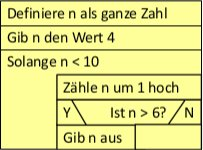
\includegraphics{mainmatter/pics/strukto.jpg}}
	\caption{ein mini Struktogramm} 
\end{figure}
%
%
%
\section{While-Schleife: Euklidischer Algorithmus}
 \begin{lstlisting}[language=JAVA]
class EuclidGCD
{
	public static void main(String... args)
	{
		int m = Integer.parseInt(args[0]);
		int n = Integer.parseInt(args[1]);
		int r = m % n;
		while (r != 0)
		{
			m = n;
			n = r;
			r = m % n;
		}
		System.out.println(n);
	}
}
\end{lstlisting}
%
%
%
\newpage
%
\section{While-Schleife: Collatzfolge (3n + 1 – Folge)}
$z_{n+1} = \left\{ \begin{array}{ll}
         \frac{1}{2}z_{n}, & z_{n}\textrm{ gerade}\\
         3 \cdot z_{n}+1, & z_{n}\textrm{ ungerade}.\end{array} \right. $\\
 \begin{lstlisting}[language=JAVA]
class CollatzMax
{
	public static void main(String... args)	
	{
		int z = Integer.parseInt(args[0]);
		int n = 0;
		int max = z;
		while (z != 1)
		{
			if (z%2 == 0){
				z = z/2;
			}
			else{
				z = 3*z + 1;
			}
			n++;
			if (z > max){
				max = z;
			}
		}
		System.out.println(n);
		System.out.println(max);
	}
}
 \end{lstlisting}
 %
 %
 %
 \section{Inkrement-/Dekrementoperator}
Variable ++; \qquad Variable - -;
 \begin{lstlisting}[language=JAVA]
 int a = 1;
int b = a++; // b = 1, a = 2
int c = a--; // c = 2, a = 1
 \end{lstlisting}
 \qquad\\
++Variable; \qquad - -Variable;
 \begin{lstlisting}[language=JAVA]
int a = 1;
int b = ++a; // b = 2, a = 2
int c = --a; // c = 1, a = 1
 \end{lstlisting}
 %
 %
 %
 \section{Der bedingte Operator}
 \begin{itemize}
 \item Dreistelliger "bedingter Operator" (engl. "conditional operator")
	\item Syntax: \\
		 condition? yes-expression: no-expression
	\item Beziehung zu if:\\
		 variable = condition? yes-expression: no-expression;
	\item äquivalent zu:\\
		 if (condition)\\
		. \qquad variable = yes-expression;\\
		 else\\
		. \qquad variable = no-expression;\\
\end{itemize}
%
%
%
\section{do-while}

\begin{figure} [H]
	\centering 
	\scalebox{0.3}{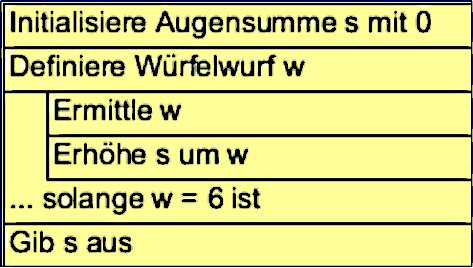
\includegraphics{mainmatter/pics/dowhile.jpg}}
	\caption{ein mini Struktogramm} 
\end{figure}

 \begin{lstlisting}[language=JAVA]
int s = 0;
int w;
do{
	w = // wuerfeln ...
	s += w;
} while (w == 6);
System.out.println(s);
 \end{lstlisting}
%
%
%
\section{Break und Continue}

\subsection{Break}
\begin{itemize}
\item Anweisung break beendet eine Schleife sofort der Rest des Rumpfes wird übersprungen
\item break = einfache Anweisung (wie Definitionen, Wertzuweisungen)
\item Zweck: Entscheidung über Fortsetzung einer Schleife fällt mitten im Rumpf
\end{itemize}

\subsection{continue}
\begin{itemize}
\item Anweisung continue startet sofort den nächsten Schleifendurchlauf der Rest des Rumpfes wird übersprungen
\item Wie break: Nützlich zur Behandlung von Sonderfällen
\item Zweck: Folge von Entscheidungen über Fortsetzung des Schleifendurchlaufes mitten im Rumpf
\end{itemize}	
Achtung: break und continue spalten Kontrollfluss: mit Bedacht
verwenden
%
%
%
\section{Gültigkeitsbereiche}
\begin{itemize}
	\item Idee
	\begin{itemize}
		\item Blöcke {...} gruppieren Anweisungen
		\item Innnerhalb eines Blocks alle Anweisungsarten erlaubt, auch Definitionen
		\item Gültigkeitsbereich (engl. „scope“) einer Variablen...
		\begin{itemize}
			\item beginnt mit der Definition und
			\item endet mit dem Block, in dem die Definition steht
		\end{itemize}
		\item Außerhalb des Blocks: Variable gilt nicht
		\item Gültigkeitsbereiche bezogen auf Quelltext, werden vom Compiler 			
			überprüft
		\item Zur Laufzeit irrelevant
	\end{itemize}
	\item Namenskollision
	\begin{itemize}
		\item Gültigkeitsbereich umfasst untergeordnete (geschachtelte) Blöcke
		\item Namenskollision: Definition des gleichen Namens, wie in einem 	
			umfassenden Block
		\item Java: Doppelte Definition unzulässig
		\item Aber: Kein Problem in disjunkten Blöcken:
	\end{itemize}
\end{itemize}
%
%
%
\section{for-Schleife}
Jede For-Schleife kann durch eine While Schleife ersetzt werden. 
 \begin{lstlisting}[language=JAVA]
for(int i = 0; i < 10; i++)
	System.out.println(i);
 \end{lstlisting}
 %
 %
 %
 \section{Switch}
 \begin{itemize}
 \item Der Wert der expression wird einmal berechnet.
\item Das Ergebnis wird nacheinander mit den labels verglichen, bis zum ersten gleichen Wert.
\item  Die dem label nachfolgenden statements werden ausgeführt, bis zum break;
\item Ziel: switch-Anweisungen ersetzen längere, unübersichtliche if-Kaskaden
\item  Syntax:
\end{itemize}
 \begin{lstlisting}[language=JAVA]
switch (expression)
{
	case label1:
		statement ...
		break;
	case label2:
		statement ...
		break;
	...
}
 \end{lstlisting}
\begin{itemize}
\item switch-Rumpf = Gültigkeitsbereich
\item Definitionen im switch-Rumpf gelten immer, nicht aber Initialisierungen
\item Unübersichtlich: besser keine Definitionen im switch-Rumpf
\item switch ist selbst eine Anweisung\\
$\Rightarrow$ kann in einem übergeordneten switch stehen
\item Nützlich um unregelmäßige Tabellen zu implementieren
\item Typ int als switch-Ausdruck zulässig
\item Nicht zulässig:
\begin{itemize}
	\item double (Test von exakten Werten problematisch $\Rightarrow$ Rundungsfehler)
	\item boolean (nur zwei Werte)
	\item ...
\end{itemize}
\item Allgemein: ganzzahlige Typen und Aufzählungstypen
\end{itemize}

 \subsection{case-Label}
 \begin{itemize}
\item case-Labels müssen eindeutig sein, doppelte Werte unzulässig
\item case-Labels müssen konstant (vom Compiler berechenbar) sein
\item  Das schließt Literale, Numerale, final-Variablen mit compiler-berechenbarem Wert und konstante Ausdrücke ein.
\item Wenn kein case-Label passt, geschieht nichts (ganzes switch wirkt wie eine leere Anweisung)
\item  Mehrere (verschiedene) case-Labels vor einer Anweisungsfolge sind zulässig
\item default = spezielles case-Label, passt auf alle übrigen Werte
\item default darf nur einmal und nur am Ende genannt werden
\item Jeder switch sollte mit einem default enden
\end{itemize}
 \begin{lstlisting}[language=JAVA]
int a = ...;
final int b = 3;
final double c = b*(b + 1);
switch(a)
{
	case 3:
	case 1 + 2:
		System.out.println("yes");
		break;
		
	case (int)c%(b - 1):
		System.out.println("maybe");
		break;
		
	default:
		System.out.println("no");
		break;
}
 \end{lstlisting}
 
 \subsection{Fall through}
 \begin{itemize}
 \item break beendet switch (zweite Anwendung von break neben Schleifen)
\item Falls break fehlt, wird mit den Anweisungen des nächsten Zweiges fortgefahren (engl. „fall through“)
\item Fall through selten sinnvoll, meistens ein Fehler, immer ein Stolperstein
\item Wenn möglich eher nicht verwenden, Programm eher umschreiben
\end{itemize}
%
%
%
\section{Klassen}
Klassen definieren neue Typen

\subsection{Klassennamen}
\begin{itemize}
\item Klassen sind mit eindeutigen Identifiern benannt
\item In der Regel englische Substantive, erster Buchstabe groß
\item Syntax:
 \end{itemize}
 \begin{lstlisting}[language=JAVA]
class Classname
{
	...
}
 \end{lstlisting}

\begin{itemize}
\item Konventionen:
	\begin{itemize}
	\item Jede Klassendefinition in einer eigenen Quelltextdatei (erzwungen bei öffentlichen Klassen)
	\item Dateiname = Klassenname + Extension .java
	\end{itemize}
\end{itemize}

\subsection{Objektvariablen}
\begin{itemize}
\item Objektvariablen sind Variablen, ebenso wie bisher verwendete Variablen
\item Zur begrifflichen Abgrenzung: bisher benutzte Variablen = lokale Variablen
\item Definitionssyntax von Objektvariablen und lokalen Variablen gleich
\item Aber: Ort der Definition unterschiedlich
\end{itemize}
\begin{tabular}{|c|c|}\hline
Objektvariablen & ... Elemente von Klassen \\ \hline
lokale Variablen & ... Anweisungen in Methoden \\ \hline
\end{tabular}
\begin{itemize}
\item Benennung von Objektvariablen:
	\begin{itemize}
	\item wie lokale Variablen
	\item eindeutig innerhalb einer Klasse
	\end{itemize}
\end{itemize}
\subsubsection{Zugriff}
\begin{itemize}
\item Jedes Objekt enthält die Objektvariablen, die in der Klassendefinition festgelegt sind
\item Objektvariablen eines Objektes können einzeln angesprochen werden: Elementzugriff
\item Objekt an das sich ein Elementzugriff richtet: Zielobjekt
\item Syntax: Zielobjekt.Objektvariable
\end{itemize}
\subsubsection{Umgang}
\begin{itemize}
\item Elementzugriff spricht Objektvariablen innerhalb eines Objektes an
\item Gleiche Verwendung wie lokale Variablen
\item Beispiel: Zähler oder Nenner eines Rational-Objektes ...
\begin{itemize}
\item  in einem Ausdruck verwenden:	int i = 5 - r.numer*3;
\item mit Operatorzuweisung und Inkrementoperator modifizieren:\\
r.numer *= 10;\\
r.numer++;
\item vergleichen: if(r.denom != 0) ...
\item usw...
\end{itemize}
\item Nur Zugriffssyntax zeigt Unterschied zwischen Objektvariablen und
lokalen Variablen
\end{itemize}
\subsubsection{Objektvariablen unterschiedlicher Objekte}
\begin{itemize}
\item Jedes Objekt hat eigene Objektvariablen (das ist der ganze Witz...)
\item Elementzugriff richtet sich an eine Objektvariable innerhalb eines Objektes (des Zielobjektes), andere Objektvariablen des Zielobjektes und Objektvariablen anderer Objekte unberührt
\end{itemize}


\subsection{Referenztypen}
\begin{itemize}
\item Classname = neuer Typ, gleichberechtigt neben primitiven Typen
\item int, double, boolean, char, byte, short, long sowie float sind primitive Typen
\item Primitive Typen sind atomar, Bausteine spielen keine Rolle
\item Gegensatz: Classname ist ein Referenztyp $\rightarrow$ enthält separate Bestandteile, diese können einzeln angesprochen und verarbeitet werden
\item Alle Klassen definieren Referenztypen
\item Auswahl primitiver Typen liegt fest, können nicht neu definiert werden
\item Erster Nutzen von Klassen: bündeln ihre Bestandteile
\end{itemize}

\subsection{Objekte / Instanzen}
\begin{itemize}
\item Klassendefinition $\approx$ Bauplan, Konstruktionsvorschrift, Blaupause
\item Objekte der Klasse müssen explizit geschaffen werden, entstehen nicht von alleine
\item  Objekt = Exemplar, Instanz
\item 1 Klassendefinition — beliebig viele Objekte
\end{itemize}

\subsection{Operator new}
\begin{itemize}
\item Erzeugen eines neuen Objektes = instanziieren (auch „konstruieren“, „allokieren“)
\item Syntaktisch mit Operator new.
\item new produziert aus einer Klassendefinition ein einzelnes, neues Objekt dieser Klasse
\item Mehrere Objekte $\Rightarrow$ mehrere Aufrufe von new
\end{itemize}
 \begin{lstlisting}[language=JAVA]
new Classname();
\end{lstlisting}

\subsection{Methoden}
\begin{itemize}
\item Methoden werden in Klassen definiert, ebenso wie Objektvariablen
\item  Objektvariablen legen Eigenschaften („Attribute“) von Objekten fest, Methoden legen Operationen fest
\item  Anders formuliert: Objektvariablen beschreiben den Aufbau von Objekten, Methoden ihr Verhalten
\item Methoden haben Namen, wie Objektvariablen (Achtung: eigener
Namensraum, Methodennamen und Objektvariablennamen clashen
nicht; aber Doppelbelegung beinahe nie sinnvoll)
\end{itemize}
 \begin{lstlisting}[language=JAVA]
class Rational
{
	int numer;
	int denom;
	
	void print()
	{
	System.out.printf("%d/%d%n", numer, denom);
	}
}
 \end{lstlisting}
 \begin{itemize}
 \item Methodendefinition = Methodenkopf + Methodenrumpf
 \item Klammern im Rumpf sind Pflicht, auch bei einer (oder keiner) Anweisung
 \begin{itemize}
 	\item nicht außerhalb einer Klassendefinition
 	\item nicht innerhalb einer anderen Methodendefinition
\end{itemize}
\item Anzahl, Reihenfolge und Anordnung von Methodendefinitionen in einer Klasse beliebig
\end{itemize}
\subsubsection{Aufruf}
\begin{itemize}
\item Methode wird mit Zielobjekt aufgerufen
\item Ohne Zielobjekt kein Aufruf (Ausnahme: statische Methoden)
\item Methodenaufruf syntaktisch ähnlich zu Elementzugriff: Zielobjekt.Methodenname();
\item Runde Klammern markieren Methodenaufruf, fehlen bei Objektvariablenzugriff
\item Ablauf eines Methodenaufrufs in mehreren Einzelschritten: Call-Sequence
\item Aufrufendes Programm („Aufrufer“, engl. caller) unterbrechen
\begin{itemize}
	\item Werte aller Argumente von links nach rechts berechnen
	\item Parameter erzeugen
	\item Parameter mit Argumentwerten initialisieren
	\item (Aufrufendes Programm („Aufrufer“) unterbrechen)
	\item (Methodenrumpf durchlaufen)
	\item Parameter zerstören
	\item (Aufrufer nach dem Aufruf fortsetzen)
\end{itemize}
\end{itemize}
\subsubsection{Methodenrumpf}
\begin{itemize}
\item Methodenrumpf = Block
\item Gültigkeitsbereich lokaler Definitionen = Methodenrumpf
\item Lebensdauer lokaler Variablen: jeweils ein Aufruf (Gegensatz Objektvariablen: Lebensdauer wie Objekt)
\item Zugriff auf Objektvariablen des eigenen Objektes ohne Angabe eines Zielobjekts
\item Ebenso: Aufruf von Methoden des eigenen Objektes ohne Angabe eines Zielobjektes
\item Methoden erreichen jede Objektvariable der eigene Klasse, unabhängig von der Anordnung der Definitionen
\end{itemize}
\subsubsection{Namenskollision}
\begin{itemize}
\item Namen von lokalen Variablen und Objektvariablen kollidieren nicht
\item Vorteil: Benennung von lokalen Variablen ohne Rücksicht auf Objektvariablen
\item Nachteil: Lokale Definition „verdeckt“ Objektvariable (oft unbeabsichtigt).
\item In der Praxis unproblematisch: Zugriffe auf Objektvariablen sowieso besser auf einzelne Methoden beschränkt (Stichwort: Datenkapselung)
\end{itemize}
\subsubsection{Parameterübergabe}
\begin{itemize}
\item Argumente und Parameter vom Compiler bei jedem Aufruf paarweise abgeglichen
\item Ein Argument pro Parameter erforderlich (zu viele oder zu wenige Argumente: wird nicht übersetzt; Ausnahme: Varargs)
\item Nötig: Typ jedes Arguments kompatibel zum entsprechenden Parameter
\item Beliebig komplizierte Ausdrücke als Argumente zulässig, werden erst ausgerechnet, dann übergeben
\item Verwendung der Parameter im Methodenrumpf: vergleichbar mit automatisch initialisierten lokalen Variablen
\item Parameter = dritte Art von Variablen, neben lokalen Variablen und Objektvariablen
\item Liste von Parametern im Methodenkopf (Komma zwischen je zwei Parametern)
\end{itemize}
%
%
%
\section{Methodenüberladung}
\begin{itemize}
\item Überladen (engl. overloading) = mehrere Methoden mit gleichen Namen, aber unterschiedlichen Parameterlisten
\item Sinnvoll für verwandte Methoden mit ähnlichem Zweck
\item Überladen mit unterschiedlicher Parameteranzahl oder unterschiedlichen Parametertypen oder beidem
\item Namen der Parameter ohne Bedeutung
\end{itemize}

\subsection{Aufruf überladener Methoden}
\begin{itemize}
\item overload resolution = Auswahl einer passenden überladenen Methode zu einer gegebenen Argumentliste — manchmal nicht ganz einfach!
\item Zuerst: Alle in Frage kommenden Kandidaten sammeln, einschließlich der Anwendung impliziter Typkonversionen
\item Unter den Kandidaten die Methode aufrufen, die am genauesten passt
\item Was bedeutet: „passt am genauesten?
\item Eine Methode a „passt genauer“ als eine Methode b, wenn jeder Aufruf von a auch von b, akzeptiert werden würde, aber nicht umgekehrt
\end{itemize}

\subsection{Mehdeutige Aufrufe: Aufrufbeispiele}
\begin{itemize}
	\item Letzter Fall: Zwei Kandidaten
\end{itemize}
\begin{tabular}{lr}
set(double, int) & nach Konversion des ersten Argumentes \\
set(int, double) & nach Konversion des zweiten Argumentes
\end{tabular}
\begin{itemize}
\item Jede der beiden Methoden akzeptiert Aufrufe, die die andere nicht akzeptiert. Keine passt genauer als die andere.
\item Der Aufruf ist mehrdeutig — Fehler
\item Methoden nur mit unterschiedlich vielen Parametern oder mit inkompatiblen Parametertypen überladen
\end{itemize}
%
%
%
\section{Ergebnisrückgabe}
\begin{itemize}
\item Mehrere return-Anweisungen im Rumpf erlaubt
\item Methode kehrt zurück, sobald zur Laufzeit das erste return erreicht wird
\item Statische Reihenfolge der return-Anweisungen unerheblich, konkreter Ablauf zur Laufzeit entscheidet
\end{itemize}

\subsection{Idee}
\begin{itemize}
\item Parameterübergabe transportiert Information vom Aufrufer zur Methode
\item Ergebnisrückgabe liefert Information von der Methode zurück zum Aufrufer
\item Eine Methode kann beliebig viele Parameterwerte annehmen, aber nur einen Ergebniswert liefern
\end{itemize}

\subsection{Definition}
Zwei gekoppelte Maßnahmen zur Ergebnisrückgabe:
\begin{itemize}
\item Typ des Ergebniswertes im Methodenkopf
\item return-Anweisung im Methodenrumpf
\end{itemize}

\subsection{Schema}
 \begin{lstlisting}[language=JAVA]
type methodname(...)
{
	...
	return expression;
}
 \end{lstlisting}
\begin{itemize}
\item Typ von expression in der return-Anweisung kompatibel zu type im Methodenkopf
\item Ausdruck „Methodentyp“ = Typ des Ergebniswertes der Methode
\item Auch kurz: „Typ-Methode“ = Methode die ein Ergebnis des Typs liefert
\end{itemize}
%
%
%
\section{Arrays}
\subsection{Motivation}
\begin{itemize}
\item Arrays (auch „Feld“, „Reihung“) vordefiniert, ohne weitere Maßnahmen verfügbar
\item Werden von praktisch allen Programmiersprachen angeboten
\item Tief in Java verankert, von der JVM intern genutzt
\item Arrays sind Containertypen: Speichern Elemente anderer Typen
\item Elementtyp beliebig, aber gleich für alle Elemente
\item Werte einzelner Elemente austauschbar
\item Anzahl Elemente eines Arrays („Arraylänge“) unveränderlich
\end{itemize}

\subsection{Arraytypen}
\begin{itemize}
\item Arrays = Familie von ähnlichen Typen, kein einzelner Typ
\end{itemize}
\begin{tabular}{l|l}
Elementtyp & Arraytyp \\ \hline
int & int[] \\
boolean & boolean[]\\
char & char[]\\
String & String[]\\
Rational & Rational[] \\
OpenCounter & OpenCounter[] \\
\end{tabular}
\begin{itemize}
\item Arraytypen sind Referenztypen
\item Ein Arraytyp legt keine Länge fest
\item Ein konkretes Exemplar eines Arrays hat eine feste, unveränderliche Länge
\end{itemize}

\subsection{Allokieren}
Erzeugen eines neuen Arrays mit einer bestimmten Anzahl Elemente eines beliebigen typs. \\
Beispiele: Arrays mit 4 bzw. 36 Elementen:
 \begin{lstlisting}[language=JAVA]
int [] a = new int[4]
Rational[] b = new Rational[3*8+12]
\end{lstlisting}
a und b referenzieren Arrays welche mit null initialisiert werden. 
\begin{itemize} 
\item Elementanzahl wird zur Laufzeit beim new-Aufruf festgelegt, kann nachher nicht mehr verändert werden
\item Elemente eines Arrays beim Allokieren automatisch mit Defaultwerten vorbesetzt (ebenso wie Objekt- und Klassenvariablen)
\item Bildhafte Vorstellung: Array = Liste namenloser Variablen, werden gemeinsam definiert, bleiben für die Lebensdauer des Arrays beisammen
\item Erzeugt nur das Array, keine Objekte, ruft keinen Element-Konstruktor auf
\end{itemize}

\subsection{Arrayliterale}
\begin{itemize}
\item Arrayliteral = Konstante eines Arraytyps
\item Allokiert neues Array aus einer Liste vorgegebener Werte
\item Schema:\\
. \qquad new type[] {expression, expression, ..., expression}
\item Länge der Arrays = Anzahl Elemente
\item  Beispiel:\\
new int[] {71, -4, 7220, 0, 238}
\item  Listenelemente = beliebige Ausdrücke, kompatibel zum Elementtyp des Arrays
\item Sinnvoll, wenn Anzahl und Werte von Elementen im Quelltext bekannt
\end{itemize}

\subsection{Elementzugriff}
\begin{itemize}
\item Elemente eines Arrays folgen linear aufeinander
\item Jedes Element hat ganzzahligen Index
\item Index des ersten Elementes = 0, dann fortlaufend weiter
\item Index des letzten Elementes = (Arraylänge − 1)
\item Zugriff auf alle Element (ungefähr) gleich schnell = random access
\item Schema für „Array-Elementzugriff“:\\
.\qquad array[expression]
\item Index zur Laufzeit berechnet aus int-Ausdruck expression
\item Zugriff auf ein Element berührt die anderen Elemente des Arrays nicht
\item Arrayelement benutzbar wie gewöhnliche Variable des Elementtyps
\item Unzulässige Indexwerte werfen ArrayIndexOutOfBoundsException
\item Negativer Index immer unzulässig
\item JVM prüft zur Laufzeit jeden Array-Elementzugriff
\item Anzahl Elemente eines Arrays (konzeptionell) beliebig
\item Erlaubt Arrays mit einem und keinem Element
\item Anzahl Elemente als öffentlich lesbare final-Objektvariable length
\item Zugriff wie Objektvariablen in Objekten:\\
array.length

\end{itemize}

\subsection{Syntax}
\begin{itemize}
\item Eckige Klammern syntaktisch in verschiedenen Kontexten
\item Typangaben:\\
Typ + leere eckige Klammern\\
int[] a;
\item Allokieren eines neuen Arrays:\\
new + Typ + Anzahl Elemente in eckigen Klammern\\
a = new int[5];
\item Array-Literal:\\
new + Typ + leere eckige Klammern + Liste von Elementen\\
a = new int[] {1, 2, 3};
\item Elementzugriff:\\
Arrayausdruck + Index in eckigen Klammern\\
a[1] = 23;
\end{itemize}

\subsection{forech-Schleife}
Kurzform einer for-Schleife für bestimmten Zweck\\
for (type variable: array)\\
statement\\
 \begin{lstlisting}[language=JAVA]
 for (int e: a){
 	...
}
\end{lstlisting}
Äquivalent zu:
 \begin{lstlisting}[language=JAVA]
for (int i = 0; i < a.length; i++){
	int e = a[i];
	...
}

\end{lstlisting}
\begin{itemize}
\item Nur Lesen, kein Schreiben des Arrays
\item Start immer mit erstem Element
\item Sequentieller Durchlauf, keine Sprünge
\item Nur ein Array, nicht mehrere parallel
\item Durchlauf abbrechen nur mit break
\end{itemize}
\subsubsection{Anwendung}
foreach geeignet für beispielsweise ...
\begin{itemize}
\item Ausgabe von Elementen
\item Suche nach Element
\item Änderungen in Elementen
\end{itemize}
 Nicht brauchbar für...
 \begin{itemize}
\item Initialisierung
\item Kopieren von Arrays
\item Vergleich zweier Arrays
\end{itemize}

\subsection{Varargs}
\begin{itemize}
\item Mit Varargs (variable length argument lists) veränderliche Anzahl Argumente möglich
\item Methodendefinition mit Vararg-Parameter
\item Vararg-Parameter syntaktisch markiert mit Typ und drei Punkten:\\
type... name
\item Beispiel:\\
int sum(int... args) \{ \}
\item Varargs ausschließlich in Parameterlisten erlaubt, nirgends sonst
\item Vararg-Parameter im Methodenrumpf verwendbar wie ein Array
\item Beispiel: int sum(int... args) ist im Rumpf der Methode gleichwertig mit int sum(int[] args)
\item Aufrufer liefert beliebig viele Argumente für einen Vararg-Parameter \\
sum(1, 2, 3)
\item Jedes einzelne Argument muß kompatibel zum Vararg-Parameter sein
\item Bei der Parameterübergabe:
\begin{itemize}
\item Allokieren eines neuen Arrays mit Länge = Anzahl Argumente
\item Initialisieren des Arrays mit Argumentwerten
\item Zuweisen des Arrays an den Vararg-Parameter
\end{itemize}
\end{itemize}
%
%
%
\section{Konstruktoren}
\begin{itemize}
\item Definition eines Konstruktors wie normale Methode, außer ...
\begin{itemize}
\item derselbe Name wie die Klasse
\item kein Vorsatz von void (oder anderem Ergebnistyp)
\end{itemize}
\item Abgesehen davon: Kopf, Parameterliste, Rumpf wie andere Methoden
\item Konstruktor mit leerer Parameterliste = Default-Konstruktor (engl. „def-ctor“)
\item new ruft automatisch Konstruktor auf
\end{itemize}
\subsubsection{Ziel:}
Automatisch sinnvoller Startzustand für neu geschaffene Objekte
\subsubsection{Idee:}
Aufruf einer normalen Methode, überladen z.B. set für Rational-Objekte
\subsubsection{Beispiel:}
leere Parameter:
\begin{lstlisting}[language=JAVA]
Rational r = new Rational();
r.set(0, 1);
\end{lstlisting}

nicht leere Parameter
\begin{lstlisting}[language=JAVA]
class Rational
{
	Rational(int n, int d)
	{
		numer = n;
		denom = d;
	}
	...
}
\end{lstlisting}
\begin{lstlisting}[language=JAVA]
Rational r = new Rational(2, 3);    // Aufruf von Rational(int, int)
r.print();   // gibt 2/3 aus
\end{lstlisting}
\begin{itemize}
\item Technisch in Ordnung, aber unzuverlässig
\item Besser: Konstruktoren (engl. „constructors“ = „ctors“):
\item Spezielle Methoden, werden automatisch bei jedem new aufgerufen
\end{itemize}

\subsection{Defaultwerten von Objektvariablen}
\begin{itemize}
\item Lokale Variablen starten nicht initialisiert (ohne Wert)
\item Gegensatz: Objektvariablen automatisch mit Defaultwerten initialisiert
\end{itemize}
\begin{tabular}{l|l}
Typ & Defaultwert \\ \hline
int & 0\\
double & 0.0\\
boolean & false \\
char & $\diagdown$u0000\\
Referenztypen & null\\
\end{tabular}

\subsection{Copy-Konstruktoren}
\begin{itemize}
\item Kopier-Konstruktor (engl. copy-ctor) erzeugt eine Kopie eines bereits existierenden Objekts
\item Vorlage (= Original-Objekt) wird als Parameter (hier: that) übergeben
\item Aufruf mit anderem Objekt als „Kopiervorlage“:
\end{itemize}
\begin{lstlisting}[language=JAVA]
Rational original = new Rational(2, 3);
Rational copy= new Rational(original);
copy.print(); // gibt 2/3 aus
\end{lstlisting}
\begin{itemize}
\item Merkmal eines Kopier-Konstruktors: Parameter der gleichen Klasse
\item Kopier-Konstruktor ausreichend für einfache Klassen, zu wenig für komplexere Klassen
\end{itemize}

\subsection{Verkettete Konstruktoren}
\begin{itemize}
\item Konstruktoren manchmal aufwändig (Tests und Vorverarbeitung von Parametern, Protokollausgaben, ...)
\item Falls mehrere überladene Konstruktoren: Kopien des gleichen Codes in jedem Konstruktor
\item Besser: Code nur in einem Konstruktor, von allen anderen mitbenutzen
\item Konstruktor-Verkettung (engl. constructor chaining) = Aufruf eines anderen Konstruktors der gleichen Klassen
\item Syntax: this als Repräsentant des „eigenen Objektes“
\item Einschränkungen verketteter Konstruktoraufrufe:
\begin{itemize}
\item this(...) muss erste Anweisung im Konstruktorrumpf sein
\item nur ein Aufruf von this(...) erlaubt
\end{itemize}
\end{itemize}

\subsection{Ergebnisrückgabe bei Konstruktoren}
\begin{itemize}
\item Definition von Konstruktoren ohne Ergebnistyp, auch nicht void
\item Resultat liegt automatisch fest: neues Objekt
\item return in Konstruktoren unzulässig
\item Keine Möglichkeit zur Rückkehr mitten aus dem Rumpf
\end{itemize}
%
%
%
\section{Klassenvariablen}
\subsection{Definition}
\begin{itemize}
\item Bisher betrachtete Objektvariablen und Methoden beziehen sich auf ein bestimmtes Objekt (= Zielobjekt)
\item Klassenvariable: einer ganzen Klasse zugeordnet, nicht einem einzelnen Objekt
\item Definiert wie normale Objektvariable + Modifier static
\end{itemize}

\subsection{Zugriff}
\begin{itemize}
\item Zugriff mit Klassennamen, statt Zielobjekt Rational.count = 0;
\item Klassenvariable existiert unabhängig von Objekten der Klasse
\item Bereits früher benutzt (Wertebereichsgrenzen, mathematische Konstanten)
\item Beispiel: Math.PI = Klassenvariable PI der Klasse Math
\end{itemize}

\subsection{Initialisierung}
\begin{itemize}
\item Initialisierung bei der Definition wie andere Objektvariablen\\
.\qquad class Rational { static int count = 0; ... }
\item Ohne explizite Initialisierung: Defaultwert abhängig vom Typ
\item Beispiel: Rational.count hätte auch ohne explizite Initialisierung den Defaultwert 0
\item Lebensdauer einer Klassenvariablen: gesamte Programmlaufzeit, unabhängig von Objekten
\end{itemize}

\subsection{Verwendung}
\begin{itemize}
\item Wichtigste Anwendung von Klassenvariablen: öffentliche Konstanten
\item Beispiele: Math.PI, Integer.MAX\_VALUE
\item Werte öffentlicher Konstanten sollen sich nicht ändern:
\begin{itemize}
\item Oft mit Modifier static und final
\end{itemize}
\end{itemize}
\begin{lstlisting}[language=JAVA]
class Integer
{
	static final int MAX_VALUE = 2147483647;
	static final int MIN_VALUE = -2147483648;
	...
}
\end{lstlisting}
\begin{itemize}
\item Konvention zur Benennung von Konstanten: ganz in Großbuchstaben, Wortteile mit Unterstrichen (\_) getrennt (anders als normale Variablen)
\item Öffentliche Konstanten werden bei der Definition initialisiert (Alternative: statische Initializer)
\end{itemize}
%
%
%
\section{Statische Methoden}
\begin{itemize}
\item Statische Methode: richtet sich an ganze Klasse, kein bestimmtes Objekt (Äquivalent zur Klassenvariable)
\item Definition mit Modifier static, sonstige Modifier und überladen wie gehabt
\item Einsatz von statischen Methoden meist als Hilfsmethoden, dieunabhängig von bestimmten Objekten sind
\item Beispiel: ggt-Methode der Klasse Rational
\end{itemize}
\begin{lstlisting}[language=JAVA]
class Rational
{
	static int gcd(int a, int b)
	{...}
}
\end{lstlisting}
\begin{itemize}
\item Kann auch ohne Rational-Objekt benutzt werden\\
System.out.println(Rational.gcd(221, 255));
\item Einige vordefinierte Klassen (z.B. Math) definieren nur statische Methoden
\end{itemize}

\subsection{main}
\begin{itemize}
\item Von Anfang an benutzt: statische Methode main = Hauptprogramm
\item Vor main existiert noch kein Objekt: main muss statisch sein
\item Wird beim Start eines Javaprogramms von der JVM automatisch in der Klasse gesucht, die auf der Kommandozeile genannt ist
\item Beispiel: Das Kommando \$java classname sucht nach der Methode
\end{itemize}
\begin{lstlisting}[language=JAVA]
class classname
{
	public static void main(String... args)
	{...}
}
\end{lstlisting}
\begin{itemize}
\item main ansonsten normale Methode: kann zum Beispiel
	\begin{itemize}
	\item überladen werden
	\item vom Programm selbst aufgerufen werden
	\item  in mehreren verschiedenen Klassen definiert sein
	\item mit einem anderen Ergebnistyp als void definiert werden.
	\end{itemize}
\end{itemize}
%
%
%
\section{Packages}
\subsection{Motivation}
\begin{itemize}
\item Pro übersetzter Bytecode-Datei (Extension .class): Bytecode einer Klasse
\item Großes Programm: Viele Bytecode-Dateien
\item Organisatorische Probleme:
\begin{itemize}
\item  Orientierung im Code
\item  Bezüge zwischen Klassen
\item Namenskonflikte zwischen gleich benannten Klassen
\item  Abgrenzung von Programmteilen
\end{itemize}
\item Vergleichbar mit Dateien auf einer Festplatte
\end{itemize}
\subsubsection{Idee:}
\begin{itemize}
\item Package = Sammlung zusammengehörender Klassen
\item Packages benannt mit Identifiern
\end{itemize}
\subsubsection{Konvetion:}
Englische Namen in kleinen Buchstaben und u.U. Ziffern, zum Beispiel utilities, project51, ...
\subsubsection{Einschärnkungen:}
\begin{itemize}
\item keine Großbuchstaben
\item keine Interpunktionszeichen
\item keine anderen Sonderzeichen
\end{itemize}
Klassennamen in unterschiedlichen Packages unabhängig, keine Kollisionen

\subsection{Packagehierarchien}
\begin{itemize}
\item Packages bilden Hierarchien (Baumstruktur)
\item in einem Package untergeordnete Packages (Sub-Packages)
\item Jedes Package in höchstens einem übergeordneten Package
\item Vergleichbar mit Verzeichnissen in einem Dateisystem
\item Packagepfad: List geschachtelter Packagenamen, getrennt mit Punkten
\item Beispiele:
\begin{itemize}
	\item project51
	\item project51.frontend
	\item project51.frontend.web
	\item project51.frontend.text
\end{itemize}
\item Innerhalb eins Packages eindeutige Namen für alle "Bewohner":
	\begin{itemize}
	\item Subpackages
	\item Klassen
	\item Enums (als spezielle Klassen)
	\item Interfaces
	\end{itemize}
\item Packagehierarchie existiert nur äußerlich: Für Java sind alle Packages gleichrangig und gleichwertig
\end{itemize}

\subsection{Dynamisches Laden von Bytecode}
\begin{itemize}
\item JVM lädt Klassen bei Bedarf (engl. on the fly), nicht beim Programmstart
\item Vorteil: Schneller Start, nicht benutzte Klassen werden überhaupt nicht geladen
\item Bedingung: Bytecode effizient lokalisierbar
\item Maßnahme: Packagepfad einer Klasse gibt Lage des Bytecodes im Filesystem vor
\ Direkte Zuordnung Packagepfad $\Rightarrow$ Directorypfad im Filesystem (nur eine Möglichkeit unter mehreren)
\item Problem:
	\begin{itemize}
	\item Packagenamen sind Java-Identifier
	\item Directorynamen sind Namen des Betriebssystems
	\end{itemize}
\item Betriebssysteme schränken Directorynamen ein $\Rightarrow$ defensive Benennungsregeln
\end{itemize}

\subsection{import-Klausel}
\begin{itemize}
\item Klassen sind mit qualifizierten Namen über Packagegrenzen hinweg ansprechbar
\item Aber: Schreibaufwändig, mühsam, fehlerträchtig
\item Einfacher mit import-Klausel:\\
import packagepath.name;
\item name im Rest des Quelltextes ohne Packagepfad nutzbar
\item Import aller Klassen eines Packages mit Jokerzeichen (engl. wildcard) *\\
import packagepath.*;
\item Joker kann nur Klassen eines Packages ansprechen $ \Rightarrow$ nur einmal und nur als letztes Element in einer import-Klausel
\item Unzulässig:
	\begin{itemize}
	\item import *.datastore;
	\item import project51.*.*;
	\end{itemize}
\item Joker schließt keine Subpackages ein
\item Mehrere import-Klauseln zulässig, Reihenfolge ohne Bedeutung
\item import-Klauseln stehen am Programmanfang, vor der Klassendefinition
\item Bezeichnung Klausel (nicht „Anweisung“): werden nur vom Compiler ausgewertet, generieren keinen ausführbaren Code
\item import-Klauseln regeln Zugriff auf andere Packages
\item Gegenstück: package-Klausel definiert Packagezugehörigkeit einer Klassendefinition
\item Syntax:\\
package packagepath;
\item Beispiel:
\end{itemize}
\begin{lstlisting}[language=JAVA]
package project51.datastore;
class Rational {...}
\end{lstlisting}
\begin{itemize}
\item package-Klausel als Erstes im Quelltext (abgesehen von Kommentar), vor import-Klauseln und Definitionen
\item package-Klausel und Pfad im Filesystem müssen übereinstimmen
\item Aufruf von Compiler und JVM mit Packagepfad
\end{itemize}

\subsection{Defaultpackage}
\begin{itemize}
\item Quelltext ohne package-Klausel: Defaultpackage (auch: „anonymes  Package“)
\item Pfad im Filesystem = CLASSPATH ohne Zusatz
\item Kein Import des Defaultpackages in andere Packages möglich (kein Name!)
\end{itemize}

\subsection{Archivdateien - Jar-Files}
\begin{itemize}
\item Bytecode in einer gepackten Archivdatei = alternative Organisationsform für Packages
\item Archivformat Jar (java archive), Dateien = „Jar-Files“, Extension .jar
\item Technisch: Zip-Files mit Erweiterungen
\item Vorteile gegenüber Directories:
	\begin{itemize}
	\item Leicht zusammen zu halten
	\item Kompression für effiziente Übertragung
	\item Metainformation bzgl. Inhalt
	\end{itemize}
\item Nachteile:
	\begin{itemize}
	\item Kein direkter Zugriff auf Bestandteile
	\item Kompression und Expansion kostet Rechenzeit
	\end{itemize}
\item Packagehierarchie in Jar-Files unverändert
\item JVM findet Bytecode in Jar-Files
\item Jar-Files im CLASSPATH: Gleichrangige Eintrittspunkte für Packagepfade\\
 CLASSPATH=/somewhere/project51.jar
\item Dateien aller Arten in Jar-Files erlaubt, JVM wertet dann nur Bytecode aus
\item Kommandozeilenwerkzeug jar zur Bearbeitung von Jar-Files
\item Aufgaben:
	\begin{itemize}
	\item  jar -cf jarfile file file ...\\
	Packt die angegebenen Dateien in ein neues Jarfile (c = create).\\
	Jokerzeichen sind erlaubt, Directories werden rekursiv eingepackt.
	\item  jar -tf jarfile\\
	Liste des Inhalts (t = table of content)
	\item  jar -xf jarfile, jar -xf jarfile file file ...\\
	Packt alle bzw. die angegebenen Dateien aus (x = extract). Directories werden rekonstruiert.
	\end{itemize}
\item Aufruf mit zusätzlichen Schalter v (= verbose): Protokollausgaben auf dem Bildschirm
\item Aufruf ohne Parameter: kurze Bedienungsanleitung
\item Metainformation (= Verwaltungsdaten, Information über das Jarfile) in der Datei META-INF/MANIFEST.MF
\item Textdatei mit Zeilen der Form \\
name:value
\item Wird automatisch angelegt mit Standard-Einträgen der Art\\
Manifest-Version: 1.0\\
Created-By: 1.5.0\_04 (Sun Microsystems Inc.)
\item Viele Einträge mit fester Bedeutung
\item Zusätzliche Einträge erlaubt
\end{itemize}
%
%
%
\section{Rekursion}
\subsection{Rekursion = Definition einer Funktion durch sich selbst}
\begin{itemize}
\item  Rekursive Definitionen erlauben oft intuitive und elegante Formulierungen von Problemen und Algorithmen
\item Für uns nur sinnvoll: wohldefinierte rekursive Definitionen, rekursiver Abstieg bis zu einer Basisdefinition
\item Verwandt mit Induktion
\end{itemize}
\subsection{Beispiel: Sum(n) := Summe der Zahlen 1..n}
$Sum(n) = \left\{ \begin{array}{ll}
         1,n =1 &\\
         n+Sum(n-1) & \textrm{sonst}.\end{array} \right. 
$\\
\begin{lstlisting}[language=JAVA]
class RecursiveSum
{
	static int recursiveSum(intSum(n) = n + Sum(n-1)
	{
		int result = (n==1) ? 1 : n + recursiveSum(n-1);
		return result;
	}
	public static void main(String... args)
	{
		int n = Integer.parseInt(args[0]);
		int sum = recursiveSum(n);
		System.out.printf("Summe von 1...%d ist %d\n", n, sum);
	}
}
\end{lstlisting}

\subsection{Beispiel: Fibonacci-Zahlen}
$F(n) := \left\{ \begin{array}{ll}
         0,n =0 &\\
         1,n =1 &\\
         F n − 1 + F(n − 2), \text{sonst}.\end{array} \right. 
$\\
\begin{lstlisting}[language=JAVA]
class Fibonacci
{
	static int fibonacci(int n)
	{
	if (n == 0)
		return 0;
	else if (n == 1)
		return 1;
	else return fibonacci(n-1) + fibonacci(n-2);
	}
	public static void main(String... args)
	{
	int n = Integer.parseInt(args[0]);
	int fib_n = fibonacci(n);
	System.out.printf("Fibonacci(%d) = %d\n", n, fib_n);
	}
}
\end{lstlisting}

\subsection{Divide \& Conquer}
Bisher:
\begin{itemize}
\item teile Problem in mehrere kleinere Teile
\item löse diese getrennt
\item setze sie wieder zusammen
\end{itemize}
Idee: Wende dieses Verfahren rekursiv auf die Teilprobleme an, bis triviale Instanzen entstehen!\\
Extrem wichtiges Verfahren im Algorithmenentwurf, erlaubt oft elegante Formulierung und effiziente Lösung!

\subsection{Effizienz:}
\begin{itemize}
\item Rekursive Aufrufe können erhebliche Laufzeitkosten bewirken!
\item Bei großen Problemen oft sinnvoll: rekursive Formulierung (besseres Verständnis) aber iterative Implementierung (oft höhere Effizienz)
\item Bestimmte Klassen rekursiver Funktionen lassen sich automatisch in Schleifen (iterative Funktionen) überführen
\item Wird bei Endrekursion oft vom Compiler gemacht
\end{itemize}

\subsection{Arten/Stufen der Rekursion}
\begin{itemize}
\item Rekursive Definitionen können in verschiedene Klassen eingeteilt werden
\item Wichtige Klassifizierungen (es gibt noch mehr!):
	\begin{itemize}
	\item Lineare Rekursion
	\item Kaskadenrekursion
	\item Endrekursion
	\item Primitive Rekursion
	\end{itemize}
\end{itemize}
\subsubsection{Lineare Rekursion}
Kommt in der rekursiven Definition nur höchstens ein rekursiver Aufruf vor spricht man von linearer Rekursion \\
$\Rightarrow$ es ergeben sich Ketten von Aufrufen
\subsubsection{Kaskadenrekursion}
Kommen mehrere rekursive Aufrufe in der Definition vor spricht man von Kaskadenrekursion\\
$\Rightarrow$ Baum von Aufrufen, oft exponentielle Laufzeit
\subsubsection{Endrekursion (Tail Recursion)}
Ist nur die letzte Anweisung einer linear rekursiven Funktion ein rekursiver Aufruf spricht man von Endrekursion\\
$\Rightarrow$ Kann unmittelbar durch while-Schleife ersetzt werden und umgekehrt, wird oft vom Compiler umgesetzt
\subsubsection{Primitive Rekursion}
Nimmt bei einer linear rekursiven Funktion der natürlichen Zahlen der Parameter mit jedem Aufruf um 1 ab oder zu spricht man von primitiver Rekursion \\
$\Rightarrow$ kann unmittelbar durch for-Schleife ersetzt werden
%
%
%
\section{Unveränderliche Klassen}

\subsection{Motivation}
\begin{itemize}
\item Bereits besprochenes Problem: Methode kann unerkannt fremdes Objekt manipulieren
\item Ursache: Freier Zugriff auf Objektvariablen
\item Lösungsidee: Unveränderliche Klassen (engl. „immutable classes“)
\item lassen keine Änderungen an Objektvariablen zu
\item Folge: Lesen von Informationen aus Objekten ok, Ändern nicht möglich
\end{itemize}

\subsection{final-Objektvariablen}
\begin{itemize}
\item Modifier final für Objektvariablen blockiert Änderungen (wie bei lokalen Variablen)
\item final-Objektvariable muss einmal mit einem Wert versorgt werden
\item Zuweisung des Wertes wahlweise ...
\begin{itemize}
	\item  Im Konstruktor
	\item Bei Initialisierung
\end{itemize}
\item  Nicht ausreichend:
\begin{itemize}
\item Defaultwert
\item anderer Methodenaufruf
\end{itemize}
\item Nachfolgende Änderung unzulässig $\Rightarrow$ erster (und einziger) Wert bleibt für die gesamte Lebensdauer des Objektes konstant
\end{itemize}

\subsection{Rückgabe neuer Objekte}
\begin{itemize}
\item Problem: Änderungen von this nicht mehr möglich
\item Ausweg: Ergebnis in neuem Objekt zurückliefern, statt this zu modifizieren
\end{itemize}
%
%
%
\section{Wertesemantik}

\subsection{Definition}
\begin{itemize}
\item Wertesemantik (engl. „value semantics“) einer Klasse: Methoden lassen this und Parameter unberührt
\item Verhalten entspricht dem von primitiven Typen: Operationen lassen Operanden unberührt
\item Gegensatz: Referenzsemantik (engl. „reference semantics“): \\
Operationen können this oder Parameter-Objekte oder beide verändern
\item Zusammenfassung:
\end{itemize}
\begin{tabular}{ll}
Primitive Typen & Wertesemantik \\
Unveränderliche Klassen & Wertesemantik\\
Veränderliche Klassen & Referenzsemantik\\
\end{tabular}

\subsection{Warum Wertesemantik?}
\begin{itemize}
\item Wertesemantik ist oft vorteilhaft
\item Beispiel: Suche nach der Ursache für fehlerhaftes Objekt
\item Referenzsemantik: Jeder Methodenaufruf kommt in Betracht, muss überprüft werden
\item Beispiel: a.mult(b);\\
könnte a oder b oder keines oder beide verändern
\item Wertesemantik: Nur Konstruktoraufrufe zu prüfen
\item Methodenaufrufe können ein korrekt erzeugtes Objekt nicht mehr stören
\item Definieren Sie Klassen wenn möglich mit Wertesemantik (= unveränderlich)
\end{itemize}
%
%
%
\section{Kopieren und vergleichen}

\subsection{Flache Kopie}
\begin{itemize}
\item Problematisch: Klasse mit Objekten als Objektvariablen
\item  Simpler Kopier-Konstruktor mit Wertzuweisungen: dupliziert Referenzen, nicht Objekte (Aliasing)
\item  Der einfache Kopier-Konstruktor erzeugt eine flache Kopie (engl. „shallow copy“): Original und Kopie referenzieren dieselben Objektvariablen
\end{itemize}
\begin{lstlisting}[language=JAVA]
class RatRange
{
	RatRange(RatRange that)
	{
		lower = that.lower;
		upper = that.upper;
	}
	...
}
\end{lstlisting}

\subsection{Tiefe Kopie}
\begin{itemize}
\item Objektvariablen mit Kopier-Konstruktor statt Wertzuweisung kopieren
\item Äußerlich kein Unterschied
\item Erzeugt eine tiefe Kopie (engl. „deep copy“): Original und Kopie enthalten logisch gleiche, isolierte Objektvariablen:
\end{itemize}
\begin{lstlisting}[language=JAVA]
class RatRange
{
	RatRange(RatRange that)
	{
		lower = new Rational(that.lower);
		upper = new Rational(that.upper);
	}
	...
}
\end{lstlisting}

\subsection{Kopieren von Objektvariablen}
\begin{itemize}
\item Regeln zum Kopieren von Objektvariablen im Kopier-Konstruktor abhängig vom Typ:
\end{itemize}
\begin{tabular}{ll}
primitiver Typ & Wertzuweisung (Beispiel Rational)\\
Referenztyp & Kopier-Konstruktor\\
Unveränderliche Klassen & Wertzuweisung (wie primitive Objektvariablen)\\
\end{tabular}		
\begin{itemize}
\item Aber: Kopier-Konstruktor zu schwach bei Vererbung (siehe später)
\item Dort: mächtigerer Mechanismus nötig
\end{itemize}

\subsection{Vergleich von Objekten}
\begin{itemize}
\item Methode equals zum Vergleich von Objekten
\item equals erwartet anderes Objekt x als Parameter, liefert ...
\begin{itemize}
\item true wenn dieses Objekt und x logisch gleichwertig sind
\item false wenn dieses Objekt und x logisch verschieden sind
\end{itemize}
\item Was heißt „logisch gleich“?
\begin{itemize}
\item Benutzer kann Objekte nicht unterscheiden
\item ... so lange keines von beiden verändert wird
\end{itemize}
\item Gleichheit ist schwächer als Identität:
\begin{itemize}
\item zwei identische Objekte sind auch gleich,
\item zwei gleiche Objekte müssen nicht identisch sein
\end{itemize}
\end{itemize}
%
%
%
\section{Datenkapselung}
\subsection{Idee:}
\begin{itemize}
\item Modul (engl. module) = Programmteil, in Java i.d.R. eine Klasse
\item Modularisierung = Aufteilung in Module
\item Modularisierung ist Ziel bei der Konstruktion von (größeren) Programmen
\item Reduktion der Abhängigkeiten zwischen Modulen: Module leichter einzeln
\begin{itemize}
\item entwerfen
\item implementieren
\item austauschen
\item erweitern
\item testen
\item korrigieren
\item ...
\end{itemize}
\item Datenkapselung (engl. „data hiding“, „data encapsulation“): Maßnahme zur Reduktion der Abhängigkeiten
\end{itemize}

\subsection{Daten und Operationen}
\begin{itemize}
\item Datenkapselung = Verbergen von Daten hinter Operationen
\item Zugriff auf Daten nur über Operationen
\item Java (und andere objektorientierte Sprachen):
\end{itemize}
\begin{tabular}{ll}
Daten & $\leftrightarrow$ Objektvariablen\\
Operationen & $\leftrightarrow$ Methoden\\
\end{tabular}
\begin{itemize}
\item Anwender einer Klasse darf Methoden aufrufen, aber keine Objektvariablen ansprechen
\end{itemize}

\subsection{Zugriffsschutz}
\begin{itemize}
\item Modifier private begrenzt Sichtbarkeit einer Definition auf die eigene Klasse
\item Von außen kein Zugriff
\item Innerhalb der eigenen Klasse keine Einschränkung
\item private gilt für den Compiler beim Übersetzen, nicht für die JVM zur Laufzeit
\item private schottet Klassen gegeneinander ab, nicht Objekte!\\
$\Rightarrow$ Unveränderliche Klassen zusammen mit Datenkapselung einsetzen
\end{itemize}

\subsection{private-Methoden}
\begin{itemize}
\item private für alle Definitionen möglich, auch für Methoden
\item  private-Methoden von außen nicht aufrufbar, nur von Methoden der eigenen Klasse
\item Sinnvoll für Hilfsmethoden, die der Anwender nicht benutzen soll
\end{itemize}

\subsection{Getter}
\begin{itemize}
\item private-Objektvariable von außen nicht erreichbar
\item  Wert dennoch zugänglich machen: Auskunftsmethode (auch „Inspector-Methode“, „Accessor-Methode“, engl. „getter“) anbieten
\item Definition eines Getter zu einer Objektvariablen:\\
private type name;
\item nach dem Muster:
\end{itemize}
\begin{lstlisting}[language=JAVA]
type getName()
{
	return name;
}
\end{lstlisting}

\subsection{Setter}
\begin{itemize}
\item private-Objektvariablen in veränderlichen Klassen: von außen kein Zugriff, keine Veränderung möglich
\item Um dennoch Modifikation zulassen: Änderungsmethoden (auch „Modifier-Methoden“, engl. „setter“) anbieten
\item Definition eines Setter zu einer Objektvariablen \\
private type name;
\item nach dem Muster (hier this sinnvoll anwendbar):
\end{itemize}
\begin{lstlisting}[language=JAVA]
void setName(type name)
{
	this.name = name;
}
\end{lstlisting}

\subsection{Vorteile Setter/Getter}
Private Objektvariablen, Setter und Getter auf den ersten Blick unnötig kompliziert gegenüber ungeschützten, öffentlichen Objektvariablen. Einsatz von Settern und Gettern dennoch sehr sinnvoll:
\begin{itemize}
\item Kontrolle der Werte
\begin{itemize}
\item Oft nur eine Teilmenge aller Werte des Typs einer Objektvariablen zulässig
\item Beispiel Rational: denom darf nicht null sein
\item Setter können unerwünschte Werte abweisen; bei freiem Zugriff keine Kontrolle
\end{itemize}
\item Fehlersuche
\begin{itemize}
\item Setter können alle Zugriffe auf Objektvariablen protokollieren; bei freiem Zugriff keine Überwachung möglich
\end{itemize}
\item Abweichende Implementierung
\begin{itemize}
\item Tatsächliche Objektvariable hinter Setter und Getter nicht sichtbar, muss überhaupt nicht existieren
\item Entsprechende Werte können pro Aufruf neu berechnet werden; für den Anwender nicht unterscheidbar
\end{itemize}
\item Verborgene Optimierungen
\begin{itemize}
\item Mit Gettern können Maßnahmen bis zum tatsächlichen Zugriff verzögert werden
\item Beispiel Rational: Mit ungekürztem Bruch rechnen, erst beim Aufruf eines Getters wirklich kürzen
\end{itemize}
\end{itemize}
%
%
%
\section{Vererbung}
\subsection{Interfaces}
\begin{itemize}
\item Schnittstelle (engl. interface) einer Klasse:
\begin{itemize}
\item Signaturen der öffentlichen (= nicht-privaten) Methoden
\item + öffentliche (= nicht-private) Objektvariablen
\end{itemize}
\item Implementierung: alles andere
\item Intuitiv:
\begin{itemize}
\item Das Interface beschreibt, was eine Klasse bietet
\item Die Implementierung legt fest, wie sie das bewerkstelligt
\end{itemize}
\item Anwender muss nur das Interface einer Klasse kennen, um sie zu  verwenden
\item Beziehung zwischen Klassendefinition und Anwendung ähnelt Geschäftsbeziehung:
\end{itemize}
\begin{tabular}{ll}
\textbf{Java} & \textbf{Geschäftsleben} \\ \hline
Klassendefinition  & Anbieter, Lieferant \\
Anwendung einer Klasse & Kunde \\
Interface & Vertrag, vereinbarte Leistungen \\
Implementierung & Betriebsmittel, interne Maßnahmen, Geschäftsgeheimnisse \\
\end{tabular}

\subsubsection{Idee:}
\begin{itemize}
\item Interface = isolierte Schnittstelle, ohne Implementierung (siehe Datenkapselung)
\item Ähnlich wie Klassendefinition, aber mit reserviertem Wort interface statt class
\item Im Interface fehlen Rümpfe der public-Methoden (statt dessen nur „;“) andere als public-Methoden, Konstruktoren, Objektvariablen (außer öffentlichen Konstanten)
\end{itemize}
\begin{lstlisting}[language=JAVA]
interface Complex
{
	public double getReal();
	public double getImag();
	public double getDistance();
	public double getPhase();
	public Complex add(Complex that);
	public Complex mult(Complex that);
	...
}
\end{lstlisting}

\subsubsection{Interface vs. Klasse}
\begin{itemize}
\item Interface ≈ Vertrag, aber Interface ≠ Klasse
\item Legt nur Anforderungen fest, liefert keine Implementierung
\item Keine Objekte von Interfaces möglich!
\item Wie bei Klassen: Eine Interfacedefinition pro Quelltextdatei, \\
Dateiname = Interfacename + .class
\item Beispiel: Interface Complex in der Quelltextdatei Complex.java
\item Bytecode: ohne ausführbare Anweisungen
\item Elemente eines Interfaces implizit public, alles andere unzulässig
\end{itemize}

\subsubsection{Implementieren von Interfaces: Klasse zum Interface}
\begin{itemize}
\item Isoliertes Interface nutzlos
\item Konkrete Klassen implementieren das Interface = definieren die Methoden des Interface
\item implements koppelt Klasse mit Interface.
\item Schematisch:\\
class Name implements Interface\\
{\\
.\qquad...\\
}
\item Klassendefinition ansonsten normal
\item Implementierung von Interfaces in einer Klasse \\
class Polar implements Complex {...}
\item Interfaces kennen keine konkreten Objekte, keine Objektvariablen\ $\Rightarrow$ können keine Konstruktoren besitzen
\end{itemize}

\subsubsection{Interfaces als Typen}
\begin{itemize}
\item Interfaces sind Typen, ebenso wie Klassen
\item Zulässig für Variablendefinitionen, Parameterlisten, Methodenergebnis, Arrayelemente, ...
\item Beispiel: Variable c vom Typ Complex\\
Complex c;
\item Objekte des Interface gibt es nicht. Was könnte c überhaupt zugewiesen werden?
\item Alle implementierenden Klassen kompatibel zum Interface
\item Beispiel: An c kann ein Cartesian-Objekt zugewiesen werden:\\
Complex c = new Cartesian(1, 2);
\end{itemize}

\subsubsection{Methodenaufrufe}
\begin{itemize}
\item Methodenaufruf mit Variable von Interfacetyp uneindeutig
\item Im allgemeinen Fall: Der Compiler kann keine getReal-Methode auswählen!
\end{itemize}

\subsubsection{Dynamisches Binden}
\begin{itemize}
\item Auswahl einer konkreten Methode fällt erst zur Laufzeit, der Compiler trifft keine Entscheidung
\item JVM sucht pro Aufruf eine Methode des momentan zugewiesenen Objekts
\item Bezeichnung: Dynamisches Binden = Zuordnung Aufruf ↔ Rumpf zur Laufzeit (weitere Form des Polymorphismus)
\end{itemize}

\subsubsection{Statischer vs. Dynamischer Typ}
\begin{itemize}
\item Dynamischer Typ = Typ des tatsächlich an eine Variable zugewiesenen Objekts\\
Complex c = new Cartesian(1, 2);
\item c hat den ...
\end{itemize}
\begin{tabular}{ll}
statischen Typ & Complex (gemäß Variablendefinition) \\
dynamischen Typ & Cartesian (das tatsächlich zugewiesene Objekt)\\
\end{tabular}
\begin{itemize}
\item Der ...
\begin{itemize}
\item statische Typ bleibt immer gleich
\item dynamische Typ kann sich ändern
\end{itemize}
\item Beim Übersetzen ist der statische Typ entscheidend (Compiler)
\item Zur Laufzeit ist der dynamische Typ entscheidend (JVM)
\end{itemize}

\subsubsection{Einsatz von Interfaces}
\begin{itemize}
\item Entwicklung, Modifikation von Interface-Implementierungen ohne Rücksicht auf andere Klassen zum gleichen Interface
\item Beispiel: neue, dritte Implementierung komplexe Zahlen namens Perplex:
\item Existenz von Cartesian und Polar kann vollkommen ignoriert werden
\begin{itemize}
\item Anwenderprogramme können sofort mit Perplex arbeiten
\item  Reibungsloses Zusammenspiel automatisch sichergestellt
\end{itemize}
\end{itemize}

\subsection{Vererbung}
\subsubsection{Code kopieren}
\begin{itemize}
\item Ergebnis: Zwei isolierte Klassen ohne Bezug
\item Problem: Fehler im Code von OpenCounter auch in MemCounter, muss zweimal identisch korrigiert werden
\item Idee: Gemeinsames Interface für OpenCounter und MemCounter
\item Jetzt: Verwandtschaft im Code dokumentiert
\item Aber: keine Hilfe bei Fehlerkorrektur
\end{itemize}

\subsubsection{Begriffe}
\begin{itemize}
\item Neuer Mechanismus: Ableitung (derivation) einer zugrunde gelegten, einfacheren Klasse zu einer erweiterten Klasse
\item Bezeichnungen:
\begin{itemize}
\item zugrunde liegende Klasse = Basisklasse (base class, super class)
\item erweiterte Klasse = abgeleitete Klasse (derived class)
\end{itemize}
\item OpenCounter = Basisklasse
\item MemCounter = abgeleitete Klasse
\item Auch Vererbung (inheritance): MemCounter erbt von OpenCounter
\item Achtung: keine Mehrfachvererbung (Mehrfachableitung) möglich!
\item Aber: Kombination mit Interface-Implementierung erlaubt!
\end{itemize}

\subsubsection{Abgeleitete Klassen}
\begin{itemize}
\item Definition einer abgeleiteten Klasse reduziert auf Unterschiede zur Basisklasse
\item Syntax einer abgeleiteten Klasse Derived:\\
class Derived extends Base ...
\item Ableitung ist asymmetrisch:
\begin{itemize}
\item Die abgeleitete Klasse kennt ihre Basisklasse (siehe Syntax)
\item Eine Basisklasse weiß nichts von abgeleiteten Klassen
\end{itemize}
\end{itemize}

\subsubsection{Ableiten zur Modifikation}
\begin{itemize}
\item Abgeleitete Klasse kann Methoden redefinieren (= neu definieren, überschreiben), die bereits in der Basisklasse definiert sind
\item Regeln:
\begin{itemize}
\item Methodenname und Typen in Parameterliste müssen exakt übernommen werden (Parameternamen dürfen geändert werden!)
\item der Zugriffsschutz darf gelockert werden
\item Der Ergebnistyp darf vom Ergebnistyp der redefinierten Methode abgeleitet sein
\item  Der Rumpf kann komplett ersetzt werden
\end{itemize}
\item Die Basisklasse wird hier nicht erweitert (wie im Beispiel MemCounter), sondern verändert
\end{itemize}

\subsubsection{Einschränken einer Basisklasse}
\begin{itemize}
\item Abgeleitete Klassen können die Funktionalität Basisklasse erweitern oder ändern, aber keinesfalls einschränken
\item Kein Sprachmittel zum Ausblenden ererbter Methoden oder Objektvariablen
\item Fazit: Ein abgeleitetes Objekt kann alles, was ein Basisklassenobjekt kann, möglicherweise auch mehr, aber keinesfalls weniger
\end{itemize}

\subsubsection{Aufruf des Basisklassen-Konstruktors}
\begin{itemize}
\item Jeder Konstruktor einer abgeleiteten Klasse muss zuerst einen Basisklassen-Konstruktor aufrufen
\item Folge: Basisklassenobjekt vollständig initialisiert, wenn abgeleiteter Konstruktor abläuft
\item Voreinstellung: Default-Konstruktor der Basisklasse
\item Basisklassen-Default-Konstruktor explizit aufrufen mit super();
\item Einschränkungen des Aufrufs von super:
\begin{itemize}
\item nur ein Aufruf
\item erste Anweisung im Konstruktorrumpf
\end{itemize}
\item super in normalen Methoden referenziert Basisklassenobjekt als Zielobjekt (weitere Nutzung von super, unabhängig vom Aufruf eines Basisklassen-Konstruktors)
\item super startet die Suche nach einer passenden Methode (dynamisches Binden) in der Basisklasse, statt in der eigenen Klasse
\item Keine Verkettung von super: spricht nur das unmittelbare Basisklassenobjekt an, kann die Basisklasse der Basisklasse nicht erreichen
\end{itemize}

\subsubsection{Anonyme Klassen}
Anonyme Klassen sind lokale Klassen mit ein paar Besonderheiten, u.A.:
\begin{itemize}
\item Ist ihr Typ nur im lokalen Block bekannt
\item Implementieren sie nie einen Konstruktor (andere lokale Klassen dürfen das)
\item Können sie auf statische Variablen der umgebenden Klasse zugreifen (auch auf private-markierte)
\item Können sie auf Objektvariablen der umgebenden Klasse zugreifen (auch auf private-markierte!), wenn sie in einer nicht-statischen Methode definiert wurden
\end{itemize}

\section{GUI}
\begin{itemize}
\item Java enthält umfangreiche Packages für die Programmierung von Benutzeroberflächen (GUI)
\item Grundidee: Package enthält Methoden, Klassen und Schnittstellen für typische Bedienelemente und Aufgaben in Benutzeroberflächen
\item Klassenhierarchie für Bedienelemente: alle Bedienelemente abgeleitet von Basisklasse oder Interface, Package kann Liste von Bedienelementen verwalten
\item Bedienelemente „wissen“ z.B. (d.h., bieten eine Methode an) wie sie sich selbst zeichnen
\item Benutzer kann solche Elemente erweitern oder implementieren und auf verschiedene Arten kombinieren
\end{itemize}

\subsection{Die Container-Klassen in Swing}
\begin{itemize}
\item Container gruppieren User-Interface-Elemente \\
$\Rightarrow$ Ein oder mehrere UI-Elemente können in einem Container platziert werden
\item JFrame:\\
Startpunkt graphischer Interfaces; ein Fenster oder Rahmen für die UI-Elemente; enthält z.B. eine Menüleiste und Toolbar, sowie einen Platz für weitere UI-Elemente (ContentPane)
\item JDialog:\\
Dialogfenster, erlaubt Abfragen an Benutzer
\item JComponent 
\begin{itemize}
\item JComponent stellt eine Basisklasse für UI-Elemente zur Verfügung, mit denen der Benutzer interagieren kann.
\item Container können JComponents enthalten und über LayoutManager anordnen
\item Jede JComponent ist auch Container \\
$\Rightarrow$ JComponents können andere JComponents enthalten
\end{itemize}
\item JPanel stellt einen Rahmen für weitere UI-Elemente zur Verfügung, der in einen Container integriert werden kann\\
 Jedes JPanel kann anderes Layout verwenden (z.B. horizontal oder vertikal) \\
$\Rightarrow$ vereinfacht komplexe Anordnung vieler Elemente in einem übergeordneten Container
\item JLabel zeigt statischen Text oder Bild an, oft gebraucht für Beschriftungen anderer Elemente oder Erklärungen\\
Wichtige Funktionen:
\begin{itemize}
\item void setText(String text)\\
setzt anzuzeigenden Text
\item void setIcon(Icon icon)\\
setzt anzuzeigendes Bild
\end{itemize}
\item JButton erzeugt einen Knopf für die GUI, der einen Text oder Bild anzeigt
und auf Druck reagieren kann\\
Wichtige Funktionen:
\begin{itemize}
\item void setText(String text) \\
setzt anzuzeigenden Text
\item void setIcon(Icon icon)\\
setzt anzuzeigendes Bild
\item void addActionListener(ActionListener a)\\
registriert von ActionListener abgeleitete Klasse, deren Funktionen
bei Ereignissen (z.B. Knopfdruck) aufgerufen werden
\end{itemize}
\item JTextField erzeugt einen Bereich, in den der Benutzer Text eingeben kann, der später vom Programm ausgelesen werden kann\\
Wichtige Funktionen:
\begin{itemize}
\item void setText(String text)\\
setzt anzuzeigenden Text
\item  String getText()\\
gibt angezeigten Text zurück
\item void addActionListener(ActionListener a)\\
registriert von ActionListener abgeleitete Klasse, deren Funktionen bei Ereignissen (z.B. Texteingabe) aufgerufen werden
\end{itemize}
\end{itemize}
\begin{tabular}{l|l}
Komponente & Beschreibung \\ \hline
JButton & Einfacher Druckknopf\\
JCheckBox & An- bzw. abwählbare Box\\
JComboBox & Auswahlbox\\
JList & Auswahlliste\\
JRadioButton & Auswahlknopf\\
JMenu & Menüleiste\\
JSlider & Schieberegler\\
JFileChooser & Dateiauswahldialog\\
JTable &Tabellenansicht\\
\end{tabular}

\subsection{Wichtige LayoutManager: Kurzübersicht}
\begin{tabular}{l|l}
Layout & Beschreibung\\ \hline
FlowLayout &Füllt Zeilenweise mit Elementen auf, bricht automatisch bei Bedarf in neue Zeilen um\\
BoxLayout & Wahlweise zeilen- oder spaltenbasiertes Layout. Legt Objekte über- oder nebeneinander ab\\
GridLayout &  Generiert x/y – Gitter von Komponenten\\
CardLayout & Ansammlung von Tabs in einem Container\\
\end{tabular}

\subsection{Events}
\begin{itemize}
\item Events: Verbindung von Benutzerinteraktion mit eigenem Code
\item Der Benutzer kann mit der GUI interagieren, aber wie bekommt unser Code Änderungen/Interaktionen mit?
\item Grundidee: Swing überprüft in einer Schleife (unterstützt durch Betriebssystem und Windowmanager) bestimmte Zustände, z.B. Mausposition, Status der Mausknöpfe, Tastendruck usw.
\item Ereignisse (Events) werden an interessierte Parteien weitergegeben
\item Wie meldet man Interesse an und wie funktioniert die Weitergabe?
\item Hinterlegen (registrieren) einer Klasse, die das ActionListener – Interface implementiert
\item Swing bestimmt betroffene Komponenten, iteriert über hinterlegte ActionListener und ruft deren actionPerformed(ActionEvent e) – Methode auf
\end{itemize}